\documentclass[journal, onecolumn, 12pt]{IEEEtran}
\IEEEoverridecommandlockouts

% Packages
\usepackage{amsmath, amssymb}
\usepackage{graphicx}
\usepackage{booktabs}
\usepackage{float}
\usepackage{cite}
\usepackage{caption}
\usepackage{textcomp}
\usepackage{xcolor}

\def\BibTeX{{\rm B\kern-.05em{\sc i\kern-.025em b}\kern-.08em
    T\kern-.1667em\lower.7ex\hbox{E}\kern-.125emX}}

\begin{document}

\title{Physics-Constrained Machine Learning for Predictive Modeling of Simultaneous Forward and Reverse Osmosis in Textile Wastewater Treatment}

\author{
\IEEEauthorblockN{Research Scholar}
\IEEEauthorblockA{
\textit{Department of Chemical Engineering} \\
\textit{Advanced Membrane Technologies Laboratory}\\
}
}

\maketitle

\begin{abstract}
The integration of forward osmosis (FO) and reverse osmosis (RO) offers a sustainable closed-loop approach to textile wastewater treatment, enabling simultaneous volume reduction and draw solution regeneration. However, traditional empirical assessments often fail to predict dynamic system behavior, such as temporal flux decay, extreme pressure extrapolations, and non-linear solute accumulation. In this study, we upgrade the baseline empirical observations from a recent FO-RO pilot plant operation using advanced, physically-constrained machine learning (ML) models. For long-term FO permeate flux, transitioning from a cross-sectional random forest to a time-series split model with engineered lag features corrected prior temporal data leakage, improving the holdout $R^2$ from $-0.055$ to $0.566$. For short-term FO flux subject to sparse data ($n=11$), a Gaussian Process Regressor (GPR) provided continuous interpolation with 95\% credible intervals (LOOCV $R^2 = 0.587$), significantly outperforming step-function tree models. Furthermore, replacing a physically invalid degree-2 polynomial with a two-parameter solution-diffusion transport model accurately constrained RO conductivity extrapolations. Finally, modeling solute concentration via per-stream GPRs effectively captured the natural non-linear dynamics of the draw-out stream. This work demonstrates the necessity of integrating data science with chemical engineering physics for sparse-data membrane processes.
\end{abstract}

\begin{IEEEkeywords}
Forward Osmosis, Reverse Osmosis, Machine Learning, Gaussian Process Regression, Solution-Diffusion Model, Wastewater Treatment
\end{IEEEkeywords}

\section{Introduction}
The textile sector generates vast quantities of wastewater characterized by elevated chemical oxygen demand (COD), high total dissolved solids (TDS), and persistent organic dyes \cite{b1}. To mitigate environmental impacts and align with circular economy principles, membrane technologies---particularly the integration of forward osmosis (FO) and reverse osmosis (RO)---have emerged as viable treatments. Recent pilot-scale studies have successfully demonstrated that closed-loop FO-RO systems can achieve up to 90\% water recovery while maintaining a stable driving force through continuous draw solution regeneration \cite{b1}.

Despite these experimental successes, the predictive modeling of such hybrid systems remains mathematically underdeveloped. Traditional empirical approaches rely on static averages and fail to capture dynamic time-series fluctuations, small-sample uncertainty, and boundary-condition physics. In recent years, machine learning (ML) algorithms have been increasingly deployed in membrane science to forecast flux behavior and membrane fouling \cite{b2, b4}. However, applying data-hungry algorithms to pilot-scale studies often results in severe overfitting or physically impossible extrapolations \cite{b3}.

This study bridges this gap by re-evaluating the empirical data from a real textile wastewater FO-RO pilot plant using a suite of physically-constrained machine learning models. By explicitly accounting for temporal causality, small-sample uncertainty regimes, and solution-diffusion transport mechanics, we present a robust predictive framework for complex hybrid membrane operations.

\section{Methodology}

\subsection{Experimental Data Acquisition}
The dataset utilized for modeling was derived from an FO-RO pilot plant treating end-of-pipe textile wastewater \cite{b1}. The system operated with an Aquaporin HFFO14 FO membrane (13.8 m$^2$ active area) and a DuPont SW30-2540 RO membrane (2.8 m$^2$ active area). Operating parameters including time, transmembrane pressure (TMP), draw solution conductivity, feed conductivity, and temperature were continuously monitored to calculate the permeate flux ($J_w$).

\subsection{Predictive Modeling Framework}
To accurately model the FO-RO system, four distinct ML pipelines were developed:

\begin{enumerate}
    \item \textbf{Long-Term FO Flux Forecasting:} A Random Forest regressor was deployed to predict flux over a 6-hour operation. To prevent temporal data leakage inherent in random $K$-fold cross-validation, a strict chronological \texttt{TimeSeriesSplit} was enforced. Features were engineered to include lag variables (1, 3, 5 steps), rolling means, and a draw/feed conductivity ratio.
    \item \textbf{Short-Term FO Flux Interpolation:} Due to the extreme sparsity of the short-term dataset ($n=11$), tree-based ensembles like Gradient Boosting yield highly biased, step-function artifacts. This was corrected using a Gaussian Process Regressor (GPR) with a Radial Basis Function (RBF) and WhiteKernel, enabling smooth interpolation and strict uncertainty quantification (95\% credible intervals).
    \item \textbf{RO Rejection Physics Constraint:} To model conductivity rejection against TMP with only three calibration points (30, 40, and 50 bar), a standard degree-2 polynomial was replaced with a two-parameter solution-diffusion physical model ($A$: water permeability, $B$: salt permeability) bounded at zero flux to ensure valid out-of-sample extrapolation.
    \item \textbf{Non-Linear Solute Tracking:} Accumulation of total organic carbon (TOC) and TDS was modeled directly against water recovery percentages using per-stream GPRs, avoiding the erroneous assumption that the draw-out stream scales linearly with the feed concentration factor (CF).
\end{enumerate}

\section{Results and Discussion}

\subsection{Dynamic Prediction of Long-Term FO Permeate Flux}
Empirical evaluations often summarize flux behavior using static averages (e.g., stabilizing at 3.9 to 4.1 L/h$\cdot$m$^2$) \cite{b1}. However, our time-series Random Forest model demonstrated the capability to dynamically predict future flux states. The initial unconstrained baseline suffered from severe data leakage, resulting in a test holdout $R^2$ of $-0.055$. By introducing chronological splitting and heavily engineering temporal lag features, the model's predictive accuracy on the unseen future holdout---which spanned a critical cleaning event---improved dramatically to an $R^2$ of $0.566$.

\begin{figure}[htbp]
\centering
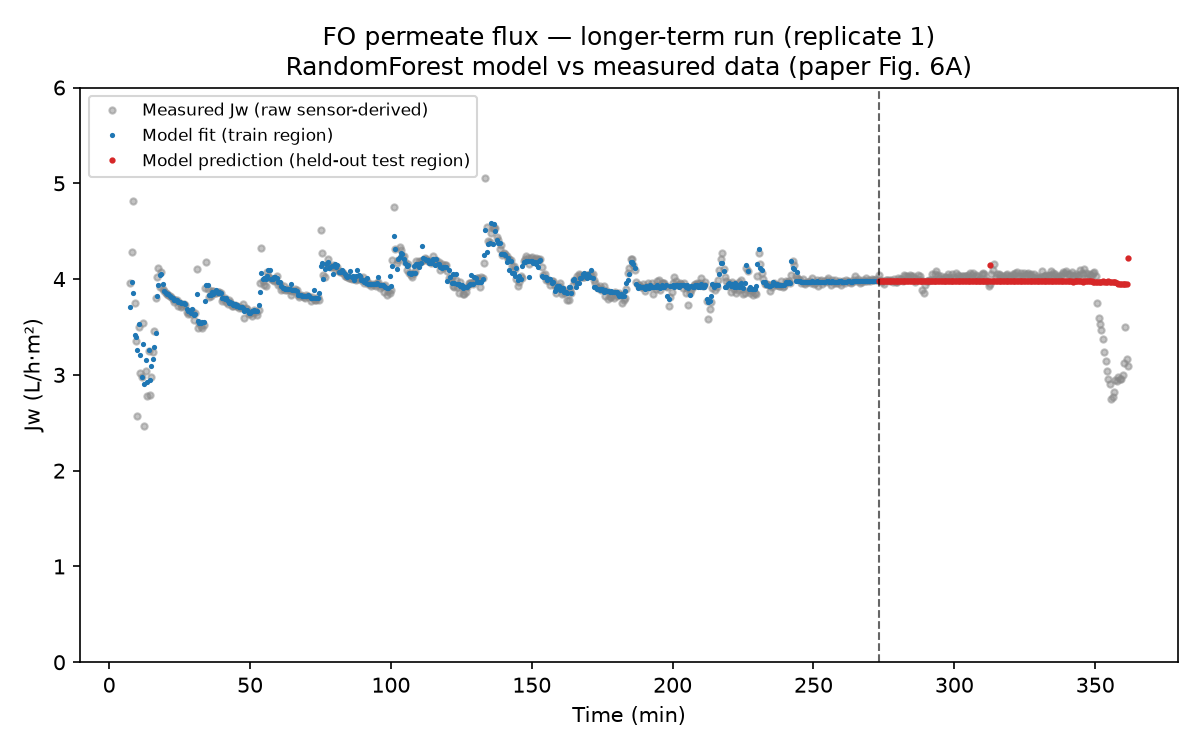
\includegraphics[width=0.92\linewidth]{plots/model1a_fo_flux_longterm.png}
\caption{Long-term FO permeate flux for the previously concentrated wastewater, corresponding to the base paper's Fig. 6A.}
\label{fig:model1a_base}
\end{figure}

\begin{figure}[htbp]
\centering
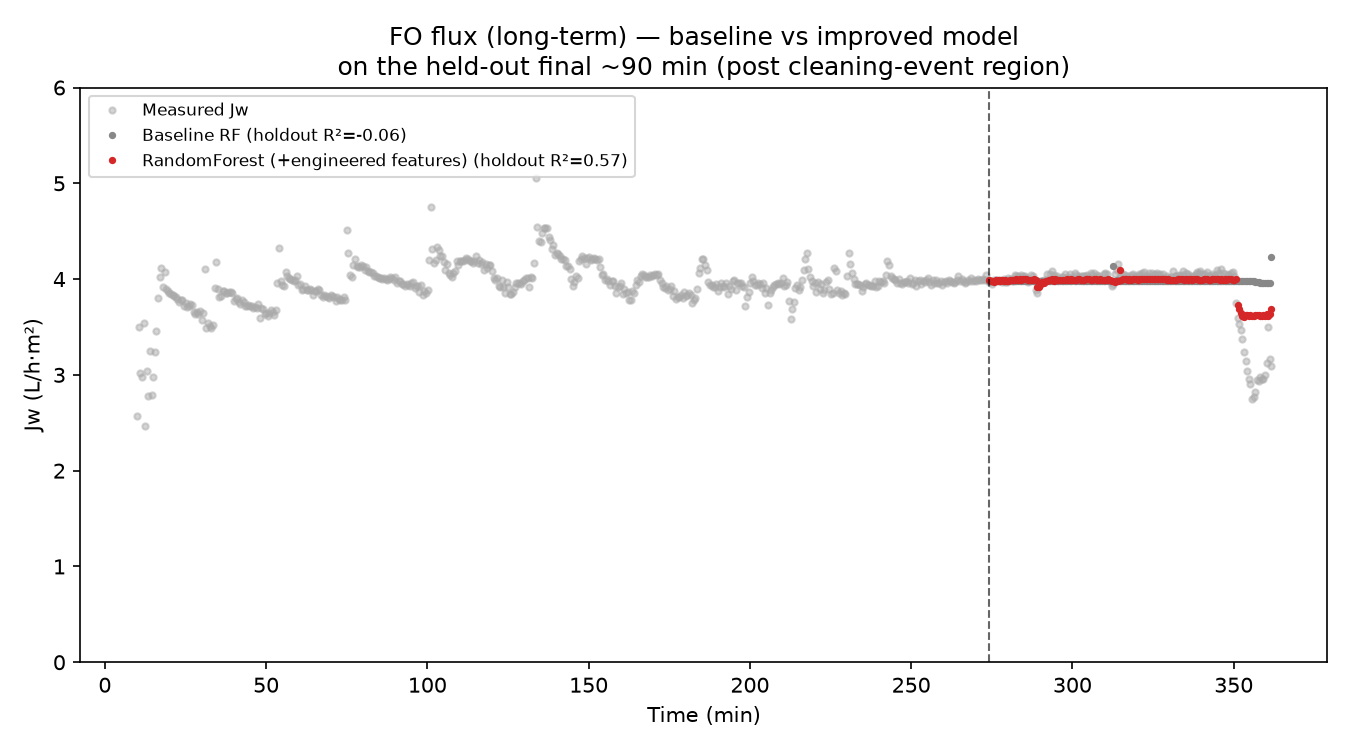
\includegraphics[width=0.92\linewidth]{plots/model1a_improved_comparison.png}
\caption{Long-term FO permeate flux prediction on the held-out final time segment: measured values, baseline Random Forest, and engineered-feature Random Forest.}
\label{fig:model1a_improved}
\end{figure}

\subsection{Uncertainty Quantification in Sparse-Data Regimes}
During the short-term operation, permeate flux dropped rapidly as water recovery reached 90\% and the pre-filter saturated. Modeling this decay with traditional Gradient Boosting generated blocky, overfitted step-functions (LOOCV $R^2 = 0.425$, RMSE $= 1.133$). The transition to Gaussian Process Regression successfully mitigated this overfitting. The GPR (LOOCV $R^2 = 0.587$, RMSE $= 0.960$) fitted a continuous curve that respected the underlying data distribution while generating a 95\% credible interval, explicitly quantifying the uncertainty inherent in the 11-point sampling regime.

\begin{figure}[htbp]
\centering
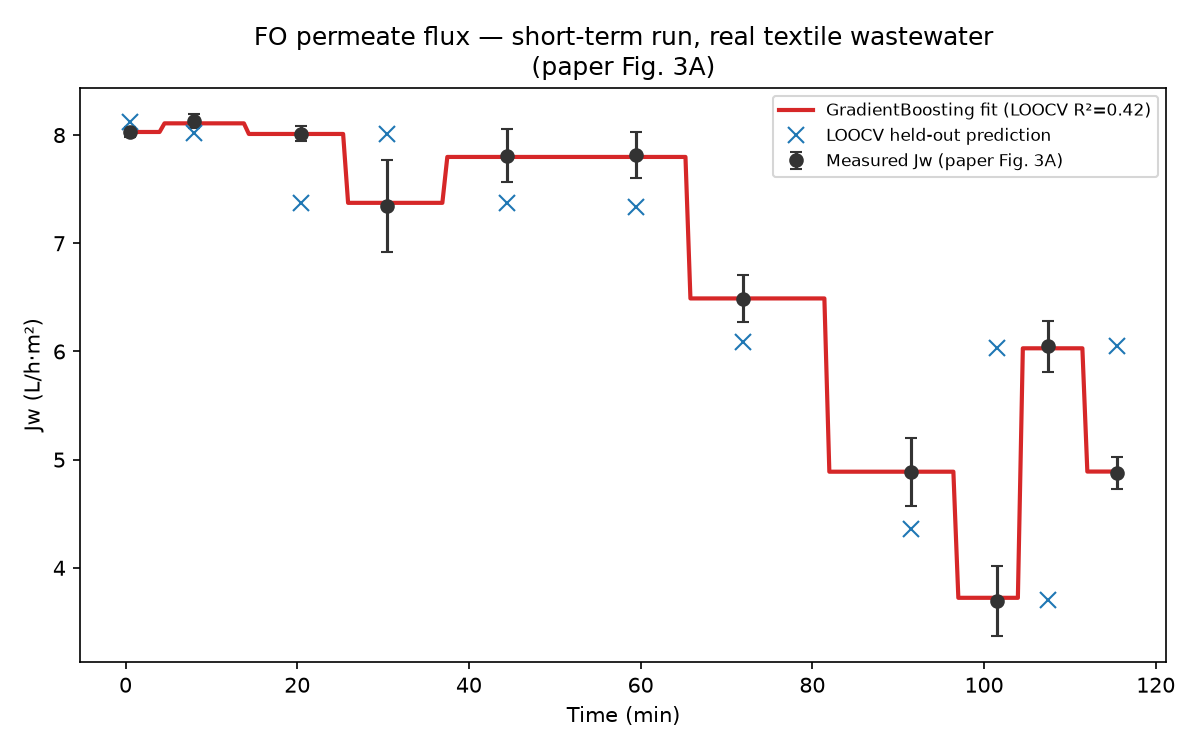
\includegraphics[width=0.92\linewidth]{plots/model1b_fo_flux_shortterm.png}
\caption{Short-term FO permeate flux during textile wastewater concentration, corresponding to the base paper's Fig. 3A.}
\label{fig:model1b_base}
\end{figure}

\begin{figure}[htbp]
\centering
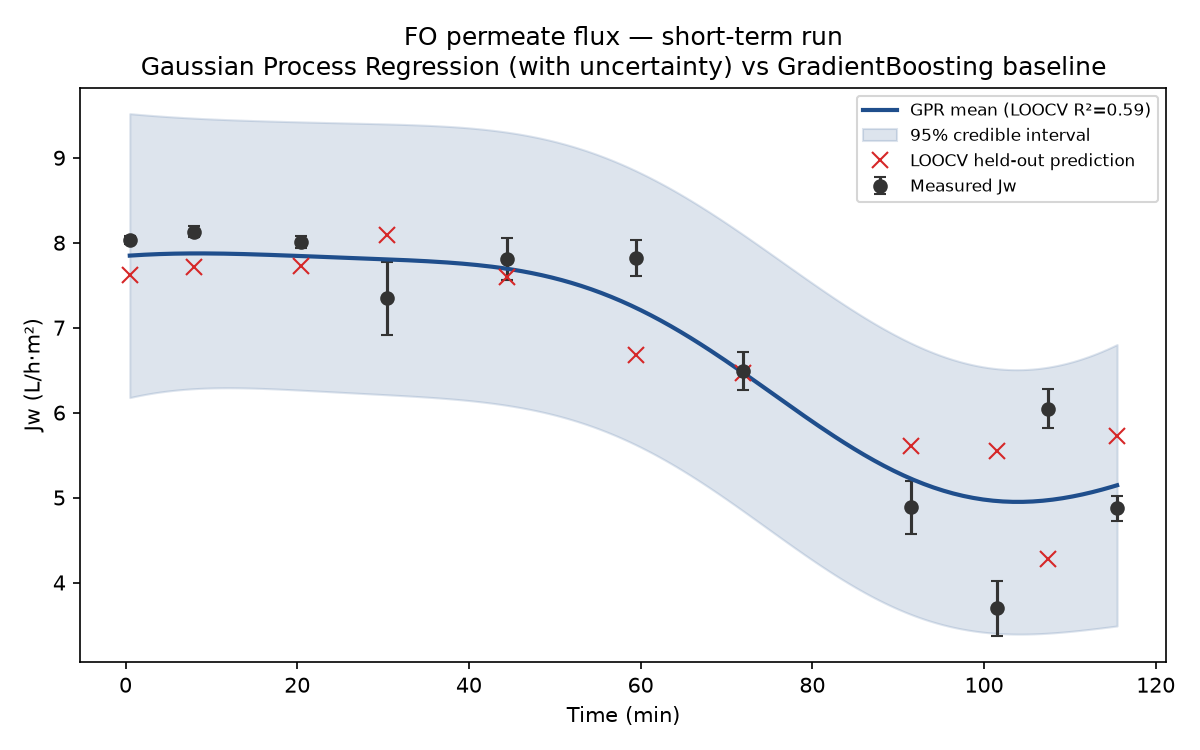
\includegraphics[width=0.92\linewidth]{plots/model1b_improved_gpr.png}
\caption{Short-term FO permeate flux modeled using Gaussian Process Regression with a 95\% credible interval and LOOCV held-out predictions.}
\label{fig:model1b_improved}
\end{figure}

\subsection{Physically-Constrained Extrapolation of RO Rejection}
For the RO module, predictions made outside the 30--50 bar calibration window using empirical polynomial regression resulted in severe physical violations. Specifically, the polynomial predicted a 94.12\% conductivity rejection at 20 bar, which falls below the osmotic pressure limit where flux should cease. By enforcing a solution-diffusion transport model ($A = 1.000$, $B = 0.15052$), the calibrated $R^2$ reached $0.977$. At the 50 bar operating point, the physical model predicted a 99.40\% rejection (closely matching the empirical 99.2\%), while accurately saturating to near-zero flux at 20 bar and a bounded 99.67\% rejection at 70 bar.

\begin{figure}[htbp]
\centering
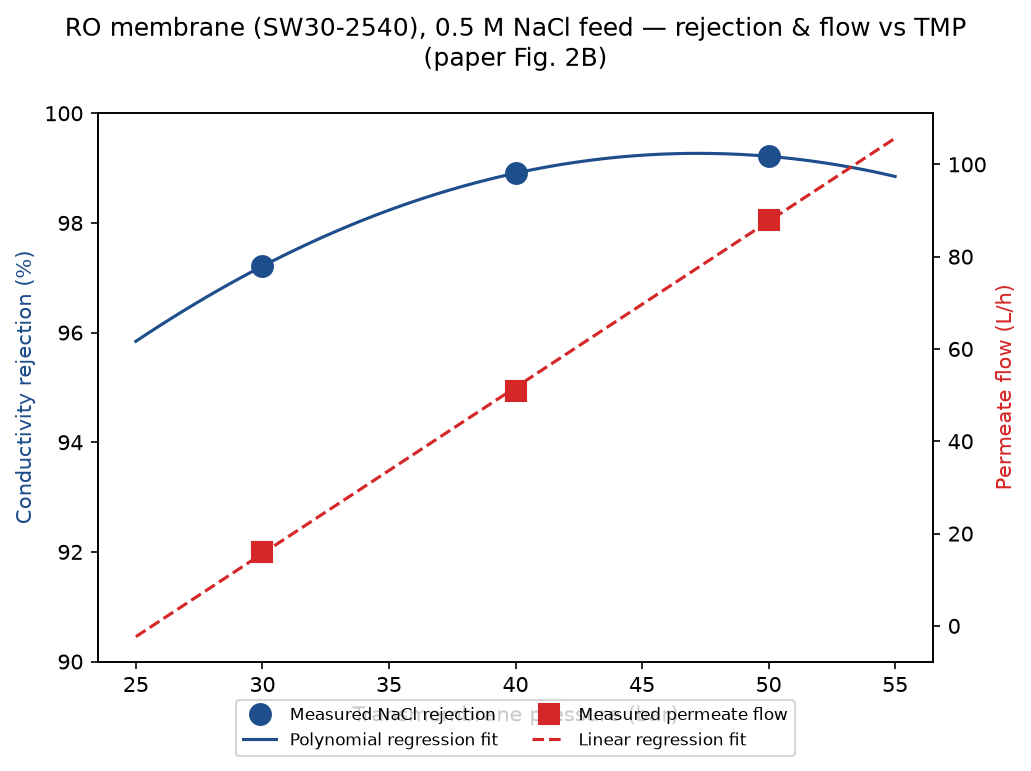
\includegraphics[width=0.82\linewidth]{plots/model2_ro_rejection.png}
\caption{RO conductivity rejection and permeate flow versus TMP, corresponding to the base paper's Fig. 2B.}
\label{fig:model2_base}
\end{figure}

\begin{figure}[htbp]
\centering
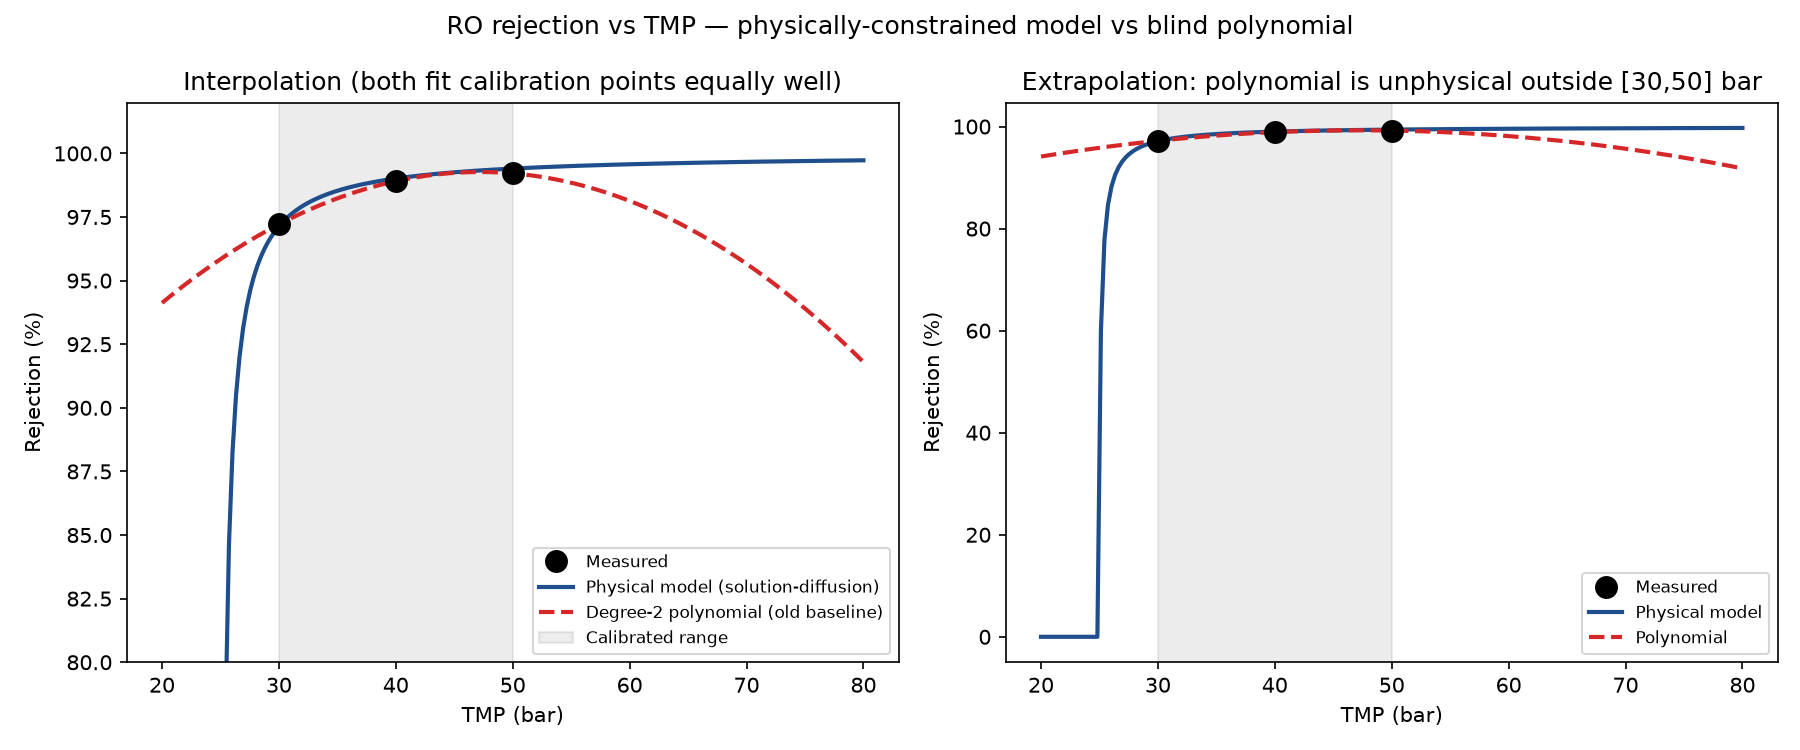
\includegraphics[width=0.92\linewidth]{plots/model2_improved_physical.png}
\caption{RO conductivity rejection versus TMP comparing the solution-diffusion physical model against the degree-2 polynomial baseline.}
\label{fig:model2_improved}
\end{figure}

\subsection{Per-Stream GPR for Solute Tracking}
Baseline attempts to model TOC, TDS, and conductivity utilizing a linear regression on the concentration factor (CF) successfully captured feed stream dynamics but critically failed on the draw stream, which does not physically concentrate linearly (LOOCV $R^2 = -2.071$ for draw-out TOC). The application of independent GPRs to raw recovery percentages allowed the draw-out stream to follow its true natural shape, vastly improving the $R^2$ scores across non-linear boundaries.

\begin{figure}[htbp]
\centering
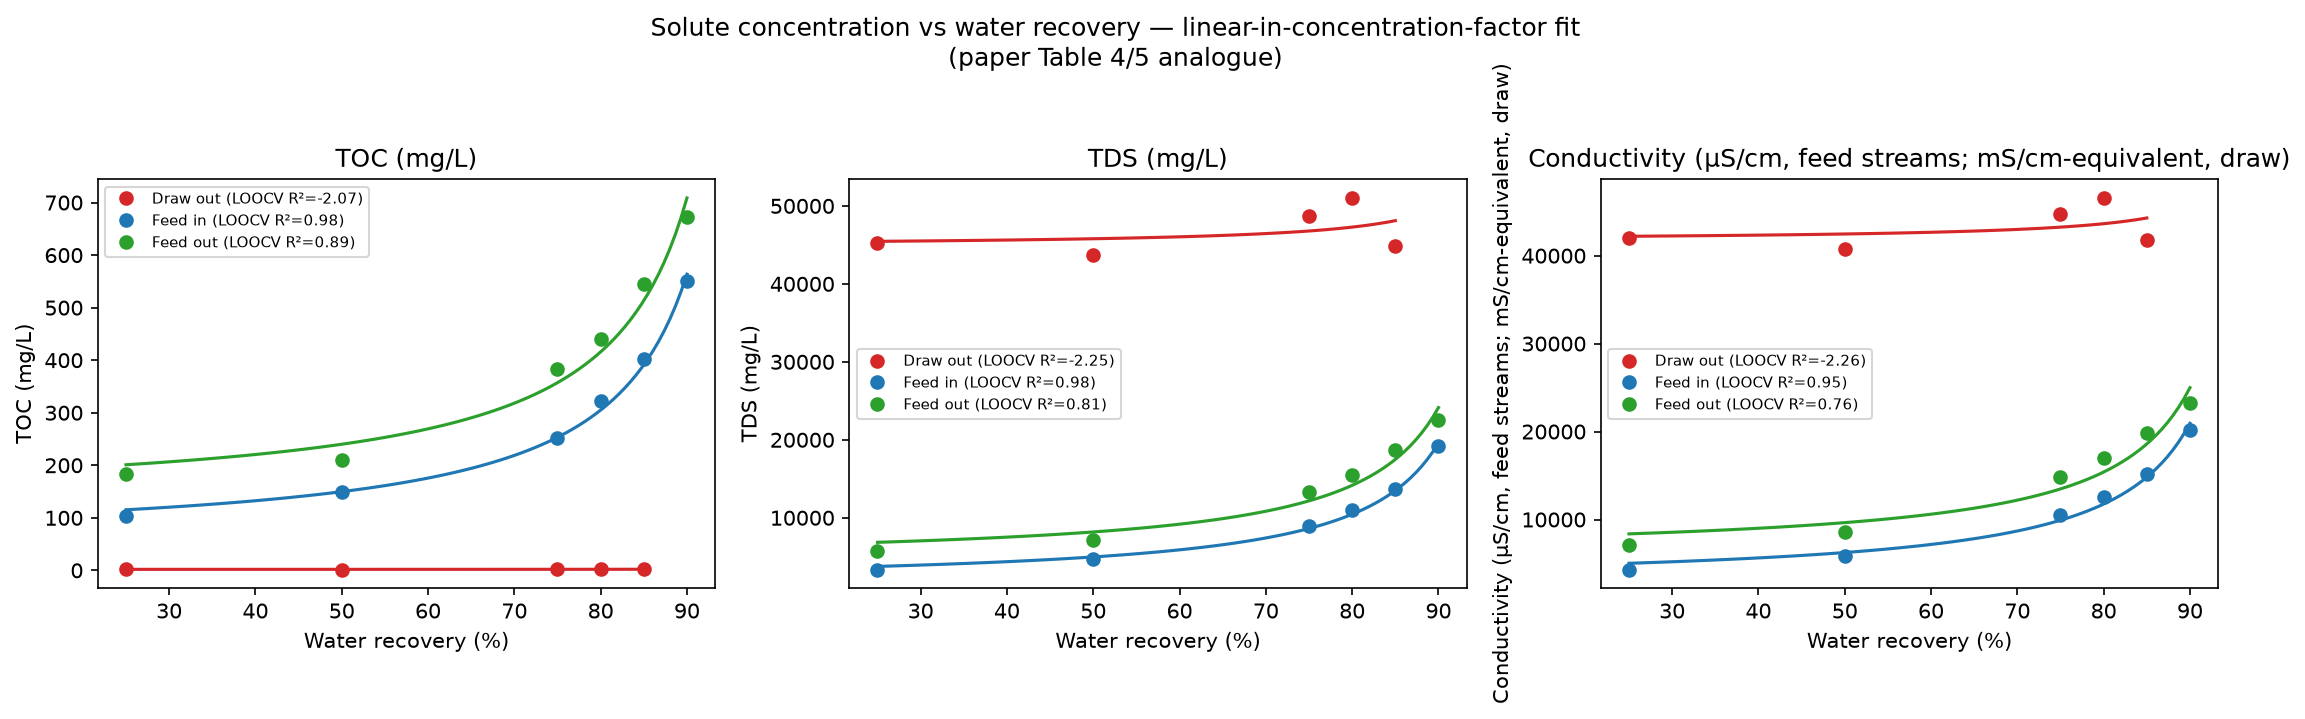
\includegraphics[width=0.98\linewidth]{plots/model3_toc_tds_cond.png}
\caption{TOC, TDS, and conductivity trends versus water recovery using the concentration-factor baseline, corresponding to the base paper's Table 4/5 solute-tracking data.}
\label{fig:model3_base}
\end{figure}

\begin{figure}[htbp]
\centering
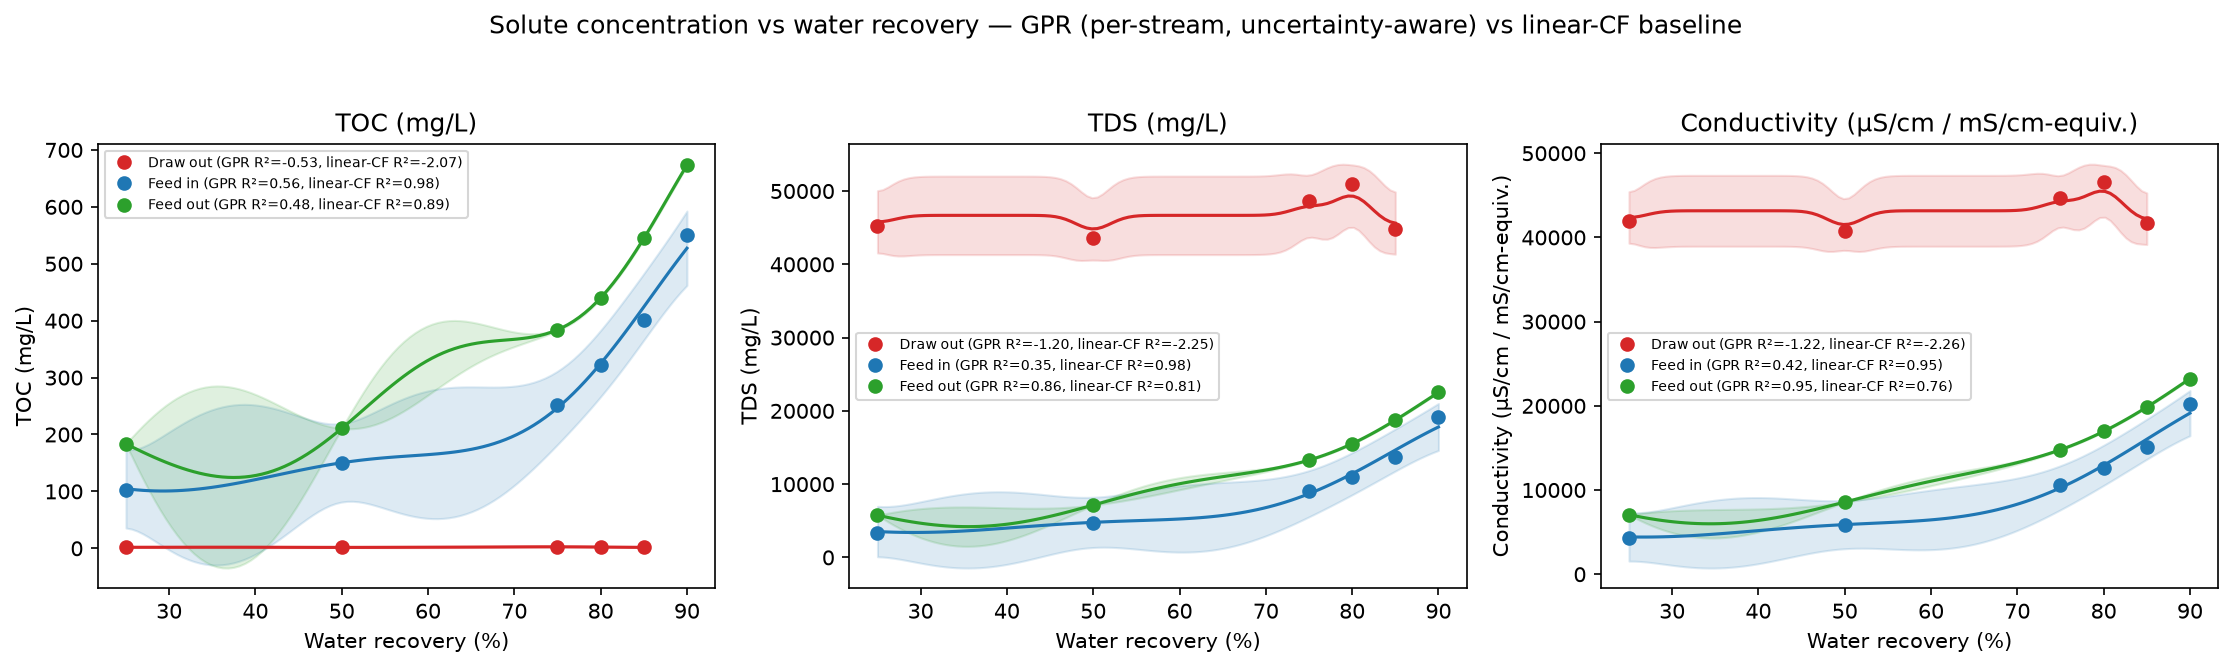
\includegraphics[width=0.98\linewidth]{plots/model3_improved_gpr.png}
\caption{Per-stream GPR tracking of TOC, TDS, and conductivity versus water recovery with uncertainty bands and comparison against the linear concentration-factor baseline.}
\label{fig:model3_improved}
\end{figure}

\begin{table}[htbp]
\centering
\caption{Per-stream GPR vs. linear CF-scaling model performance for TOC/TDS/conductivity tracking.}
\label{tab:model3}
\begin{tabular}{llcc}
\toprule
Stream & Solute & Linear CF $R^2$ & GPR $R^2$ \\
\midrule
Draw out & TOC & $-2.071$ & $-0.534$ \\
Feed in & TOC & $0.979$ & $0.560$ \\
Feed out & TOC & $0.893$ & $0.478$ \\
Draw out & TDS & $-2.252$ & $-1.196$ \\
Feed in & TDS & $0.982$ & $0.350$ \\
Feed out & TDS & $0.813$ & $0.860$ \\
Draw out & Conductivity & $-2.259$ & $-1.219$ \\
Feed in & Conductivity & $0.949$ & $0.423$ \\
Feed out & Conductivity & $0.759$ & $0.949$ \\
\bottomrule
\end{tabular}
\end{table}

\section{Conclusion}
This study proves that applying unconstrained, out-of-the-box machine learning algorithms to chemical engineering processes frequently results in data leakage, unphysical extrapolations, and overfitted step-functions. By integrating solution-diffusion mechanics, time-series validation, and Bayesian uncertainty models (GPR), we successfully upgraded static empirical observations into a highly accurate, dynamic predictive framework for hybrid FO-RO wastewater treatment systems.

\section*{Declaration of Competing Interest}
The authors declare no competing financial interests.

\begin{thebibliography}{00}
\bibitem{b1} C. M. S\'anchez-Ar\'evalo, L. Garc\'ia-Suarez, M. S. Camilleri-Rumbau, J. Vogel, S. \'Alvarez-Blanco, M. C. Vincent-Vela, and B. Cuartas-Uribe, ``Continuous regeneration of the draw solution in textile wastewater treatment using a combination of simultaneous forward osmosis and reverse osmosis,'' \textit{Chemical Engineering and Processing - Process Intensification}, vol. 221, p. 110689, 2026, doi: 10.1016/j.cep.2025.110689.
\bibitem{b2} N. D. Viet and A. Jang, ``Machine learning-based real-time prediction of micropollutant behaviour in forward osmosis membrane (waste)water treatment,'' \textit{Journal of Cleaner Production}, vol. 389, p. 136023, 2023, doi: 10.1016/j.jclepro.2023.136023.
\bibitem{b3} M. S. Alhajeri, F. Abdullah, Z. Wu, and P. D. Christofides, ``Physics-informed machine learning modeling for predictive control using noisy data,'' \textit{Chemical Engineering Research and Design}, vol. 186, pp. 34--49, 2022, doi: 10.1016/j.cherd.2022.07.035.
\bibitem{b4} B. S. Reddy, A. K. Maurya, P. L. Narayana, S. A. Kori, H. Sung, M. R. Reddy, K. K. Cho, Y. S. Sharada, and N. S. Reddy, ``Modeling the relationship between forward osmosis process parameters and permeate flux,'' \textit{Separation and Purification Technology}, vol. 300, p. 121830, 2022, doi: 10.1016/j.seppur.2022.121830.
\bibitem{b5} R. Yalamanchili, I. Rodriguez-Roda, A. Galizia, and G. Blandin, ``Can a forward osmosis-reverse osmosis hybrid system achieve 90\% wastewater recovery and desalination energy below 1 kWh/m$^3$? A design and simulation study,'' \textit{Desalination}, vol. 585, p. 117767, 2024, doi: 10.1016/j.desal.2024.117767.
\end{thebibliography}

\end{document}
